\exerciseset{In Exercises}{, sketch the vector--valued function on the given interval in $\mathbb{R}^3$. Technology may be useful in creating the sketch.}{

\exercise{$\vec r(t) = \la 2\cos t, t, 2\sin t\ra$, on $[0,2\pi]$.
}{\begin{minipage}{\linewidth}
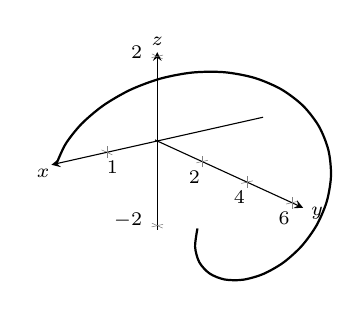
\begin{tikzpicture}[>=stealth]
\begin{axis}[width=175pt,tick label style={font=\scriptsize},axis on top,
axis lines=center,view={145}{25},name=myplot,
xtick={1},ymin=-.1,ymax=6.5,xmin=-2.1,xmax=2.1,zmin=-2.1, zmax=2.1,
every axis x label/.style={at={(axis cs:\pgfkeysvalueof{/pgfplots/xmax},0,0)},xshift=-3pt,yshift=-3pt},
xlabel={\scriptsize $x$},
every axis y label/.style={at={(axis cs:0,\pgfkeysvalueof{/pgfplots/ymax},0)},xshift=5pt,yshift=-2pt},
ylabel={\scriptsize $y$},
every axis z label/.style={at={(axis cs:0,0,\pgfkeysvalueof{/pgfplots/zmax})},xshift=0pt,yshift=4pt},
zlabel={\scriptsize $z$}]

\addplot3[domain=0:6.28,samples y=0,{\colorone},smooth,thick] ({2*cos(deg(x))},{x},{2*sin(deg(x))});

\end{axis}
%\node [right] at (myplot.right of origin)[shift={(-20pt,-8pt)}] {\scriptsize $y$};
%\node [above] at (myplot.above origin) [shift={(0,-5pt)}] {\scriptsize $z$};
\end{tikzpicture}
\end{minipage}}

\exercise{$\vec r(t) = \la 3\cos t, \sin t, t/\pi\ra$ on $[0,2\pi]$.
}{\begin{minipage}{\linewidth}
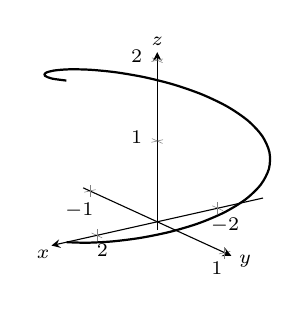
\begin{tikzpicture}[>=stealth]
\begin{axis}[width=175pt,tick label style={font=\scriptsize},axis on top,
axis lines=center,view={145}{25},name=myplot,
ymin=-1.1,ymax=1.1,xmin=-3.5,xmax=3.5,zmin=-0.1, zmax=2.1,
every axis x label/.style={at={(axis cs:\pgfkeysvalueof{/pgfplots/xmax},0,0)},xshift=-3pt,yshift=-3pt},
xlabel={\scriptsize $x$},
every axis y label/.style={at={(axis cs:0,\pgfkeysvalueof{/pgfplots/ymax},0)},xshift=5pt,yshift=-2pt},
ylabel={\scriptsize $y$},
every axis z label/.style={at={(axis cs:0,0,\pgfkeysvalueof{/pgfplots/zmax})},xshift=0pt,yshift=4pt},
zlabel={\scriptsize $z$}]

\addplot3[domain=0:6.28,samples y=0,{\colorone},smooth,thick] ({3*cos(deg(x))},{sin(deg(x))},{x/3.14159});
\end{axis}
%\node [right] at (myplot.right of origin)[shift={(-20pt,-8pt)}] {\scriptsize $y$};
%\node [above] at (myplot.above origin) [shift={(0,-5pt)}] {\scriptsize $z$};
\end{tikzpicture}
\end{minipage}}

\exercise{$\vec r(t) = \la \cos t, \sin t,\sin t\ra$ on $[0,2\pi]$.
}{\begin{minipage}{\linewidth}
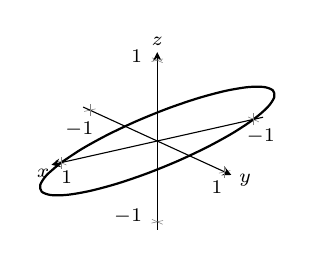
\begin{tikzpicture}[>=stealth]
\begin{axis}[width=175pt,tick label style={font=\scriptsize},axis on top,
axis lines=center,view={145}{25},name=myplot,
ymin=-1.1,ymax=1.1,xmin=-1.1,xmax=1.1,zmin=-1.1, zmax=1.1,
every axis x label/.style={at={(axis cs:\pgfkeysvalueof{/pgfplots/xmax},0,0)},xshift=-3pt,yshift=-3pt},
xlabel={\scriptsize $x$},
every axis y label/.style={at={(axis cs:0,\pgfkeysvalueof{/pgfplots/ymax},0)},xshift=5pt,yshift=-2pt},
ylabel={\scriptsize $y$},
every axis z label/.style={at={(axis cs:0,0,\pgfkeysvalueof{/pgfplots/zmax})},xshift=0pt,yshift=4pt},
zlabel={\scriptsize $z$}]

\addplot3[domain=0:6.28,samples y=0,{\colorone},smooth,thick] ({cos(deg(x))},{sin(deg(x))},{sin(deg(x))});
\end{axis}
%\node [right] at (myplot.right of origin)[shift={(-20pt,-8pt)}] {\scriptsize $y$};
%\node [above] at (myplot.above origin) [shift={(0,-5pt)}] {\scriptsize $z$};
\end{tikzpicture}
\end{minipage}}

\exercise{$\vec r(t) = \la \cos t, \sin t,\sin (2t)\ra$ on $[0,2\pi]$.
}{\begin{minipage}{\linewidth}
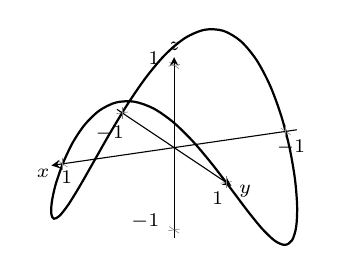
\begin{tikzpicture}[>=stealth]
\begin{axis}[width=175pt,tick label style={font=\scriptsize},axis on top,
axis lines=center,view={155}{25},name=myplot,
ymin=-1.1,ymax=1.1,xmin=-1.1,xmax=1.1,zmin=-1.1, zmax=1.1,
every axis x label/.style={at={(axis cs:\pgfkeysvalueof{/pgfplots/xmax},0,0)},xshift=-3pt,yshift=-3pt},
xlabel={\scriptsize $x$},
every axis y label/.style={at={(axis cs:0,\pgfkeysvalueof{/pgfplots/ymax},0)},xshift=5pt,yshift=-2pt},
ylabel={\scriptsize $y$},
every axis z label/.style={at={(axis cs:0,0,\pgfkeysvalueof{/pgfplots/zmax})},xshift=0pt,yshift=4pt},
zlabel={\scriptsize $z$}]

\addplot3[domain=0:6.28,samples y=0,{\colorone},smooth,thick,samples=40] ({cos(deg(x))},{sin(deg(x))},{sin(deg(2*x))});
\end{axis}
%\node [right] at (myplot.right of origin)[shift={(-20pt,-8pt)}] {\scriptsize $y$};
%\node [above] at (myplot.above origin) [shift={(0,-5pt)}] {\scriptsize $z$};
\end{tikzpicture}
\end{minipage}}

}
